\documentclass[11pt]{article}
\usepackage[margin=1in]{geometry}
\usepackage{amsmath}

\title{No way! Are you serious???}
\author{Test Author}
\date{\today}

\begin{document}

\maketitle

\section{Introduction}

This is an ultra minimal test document for texMini. $a^2 + b^2 = c^2$

\section{Basic Math}

Inline math: $E = mc^2$ and $f(x) = x^2 + 1$.

Display math:
\begin{equation}
    \int_0^1 x^2 dx = \frac{1}{3}
\end{equation}

\section{Lists}

\begin{itemize}
    \item First item
    \item Second item
    \item Third item
\end{itemize}

\begin{enumerate}
    \item Numbered item one
    \item Numbered item two
    \item Numbered item three
\end{enumerate}

\section{Conclusion}

If this compiles, texMini basic functionality works.

\end{document}
    \item Numbered item three
\end{enumerate}

\section{Colors}


Some \textcolor{red}{red text} and \textcolor{blue}{blue text}.

\section{Conclusion}


If this document compiles successfully, texMini is working correctly.

\end{document}
        a_{11} & a_{12} & \cdots & a_{1n} \\
        a_{21} & a_{22} & \cdots & a_{2n} \\
        \vdots & \vdots & \ddots & \vdots \\
        a_{m1} & a_{m2} & \cdots & a_{mn}
    \end{pmatrix}
\end{equation}

\section{Colors and Hyperlinks}

texMini includes xcolor and hyperref:

\begin{itemize}
    \item \textcolor{red}{Red text}
    \item \textcolor{blue}{Blue text}
    \item \textcolor{green}{Green text}
    \item Link to \href{https://github.com/alexmill/texMini}{texMini repository}
\end{itemize}

\section{Graphics with TikZ}

texMini includes pgf/tikz for creating graphics:

\begin{center}
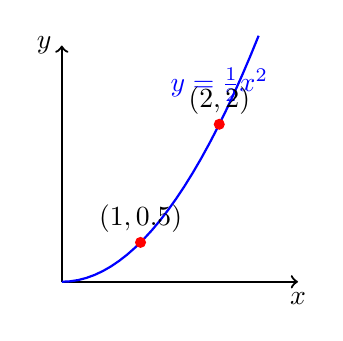
\begin{tikzpicture}
    % Draw a simple diagram
    \draw[thick, ->] (0,0) -- (3,0) node[anchor=north] {$x$};
    \draw[thick, ->] (0,0) -- (0,3) node[anchor=east] {$y$};
    
    % Draw a function
    \draw[blue, thick, domain=0:2.5] plot (\x, {0.5*\x*\x});
    \node[blue] at (2, 2.5) {$y = \frac{1}{2}x^2$};
    
    % Draw some points
    \fill[red] (1,0.5) circle (2pt);
    \fill[red] (2,2) circle (2pt);
    
    \node[anchor=south] at (1,0.5) {$(1,0.5)$};
    \node[anchor=south] at (2,2) {$(2,2)$};
\end{tikzpicture}
\end{center}

\section{Framed Content}

texMini includes the framed package:

\begin{framed}
This is content inside a frame. This tests that the framed package is working correctly with texMini.
\end{framed}

\section{Page Layout}

This document uses the geometry package to set 1-inch margins, demonstrating that page layout packages work correctly.

\section{Compilation Test}

If you can see this section and the document compiled without errors, then:

\begin{enumerate}
    \item Your Nix flake configuration is correct
    \item texMini is being pulled from GitHub successfully
    \item LaTeX Workshop is correctly invoking the texMini toolchain
    \item All the essential packages in texMini are working
\end{enumerate}

\subsection{Expected Behavior}

When you save this document in VS Code:
\begin{itemize}
    \item LaTeX Workshop should automatically build it (due to autoBuild.run = "onSave")
    \item The first build might take a moment as Nix downloads texMini
    \item Subsequent builds should be faster as texMini will be cached
    \item The PDF should open in a VS Code tab
    \item Any compilation errors should appear in the Problems panel
\end{itemize}

\section{Troubleshooting}

If this document doesn't compile:
\begin{enumerate}
    \item Check the LaTeX Workshop output panel for error messages
    \item Ensure you're running VS Code from nix run in this directory
    \item Verify that your system has network access to download texMini
\end{enumerate}

\section{Conclusion}

This test document exercises the core functionality provided by texMini. If it compiles successfully, your development environment is ready for LaTeX work with a minimal but capable TeX distribution.

The texMini approach gives you:
\begin{itemize}
    \item Fast downloads (approximately 100 MB vs approximately 5 GB for full TeX Live)
    \item Reproducible builds via Nix
    \item Essential packages for most LaTeX documents
    \item Extensibility when you need additional packages
\end{itemize}

\end{document}
